\begin{frame}{Associative Rules Analysis}{Looking for implications among the dataset's attributes}

\centering{What do we need to perform an associative analysis?} \vspace{0,4cm}

	\begin{block}{}
		\begin{itemize}
			\item<1-> \alert{Discretized data set} --- we need \emph{discrete attributes} in order to find logical implications netween them;
			\item<2-> \alert{Apriori algorithm} --- it uses an heuristic technique to render the \emph{candidate generation problem} computable;
			\item<3-> \alert{Confidence metric} --- a good choice is \textbf{lift}, as it values a rule ability to predict cases comparing it against the odds of a random prediction.
		\end{itemize}
	\end{block}

\end{frame}

\begin{frame}{Associative Rules Analysis}{Looking for implications among the dataset's attributes}

    Focus on the \alert{teaching course}: mined rules.

    \vspace{0.4cm}
    \begin{centering}
        \hspace{0.5cm}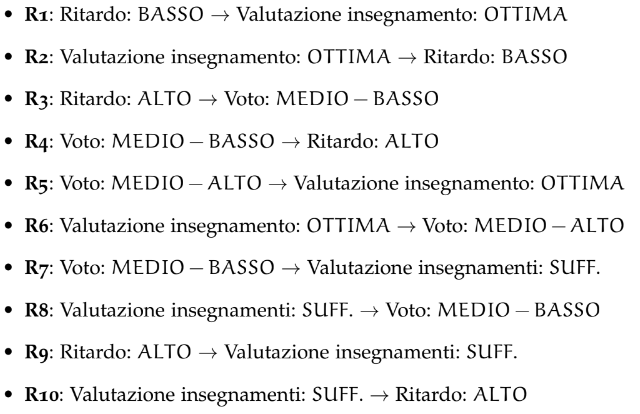
\includegraphics[scale=0.40]{ass2.png}
    \end{centering}

\end{frame}

\begin{frame}{Associative Rules Analysis}{Looking for implications among the dataset's attributes}

    \vspace{0.2cm}
    Focus on the \alert{teaching course}: rules performances.
    \vspace{0.2cm}

    \begin{centering}
        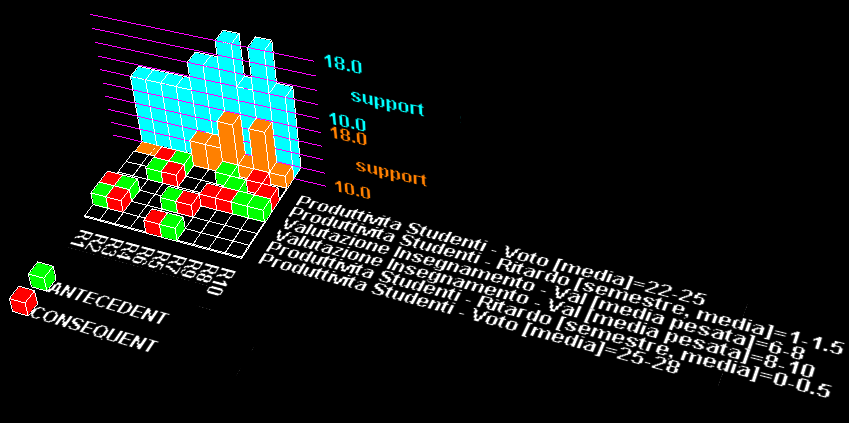
\includegraphics[scale=0.36]{../ass/apriori_min_1.png}
    \end{centering}

\end{frame}

\begin{frame}{Associative Rules Analysis}{Looking for implications among the dataset's attributes}

    Focus on the \alert{teaching course}: \emph{what have we found?}.

    \vspace{0.5cm}
    \begin{centering}
        \hspace{0.5cm}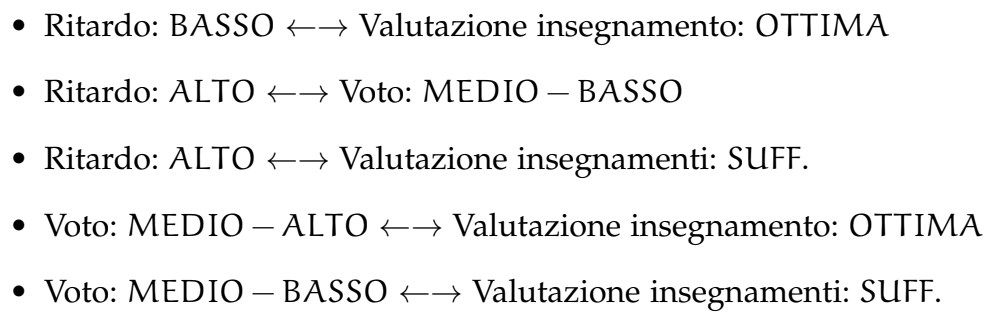
\includegraphics[scale=0.30]{ass1.png}
    \end{centering}

\end{frame}

\begin{frame}{Associative Rules Analysis}{Looking for implications among the dataset's attributes}

    Other aspects can be investigated this way: teachers related attributes, specific attributes, etc.

    \vspace{0.2cm}
	\begin{itemize}
		\item<1-> Focus on \alert{teachers}: \\ \vspace{0.2cm} 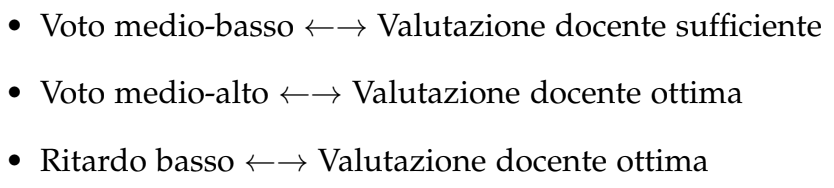
\includegraphics[scale=0.28]{ass4.png}
		\item<2-> Focus on \alert{standard deviations}: \\ \vspace{0.2cm} 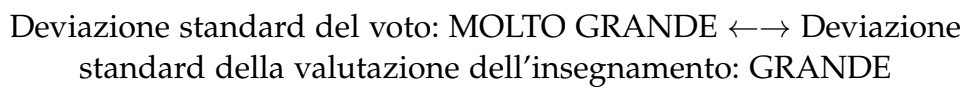
\includegraphics[scale=0.28]{ass5.png}
	\end{itemize}

\end{frame}